\subsection{Contributors} \label{repo_analysis_contributors}

\begin{figure}
    \centering
    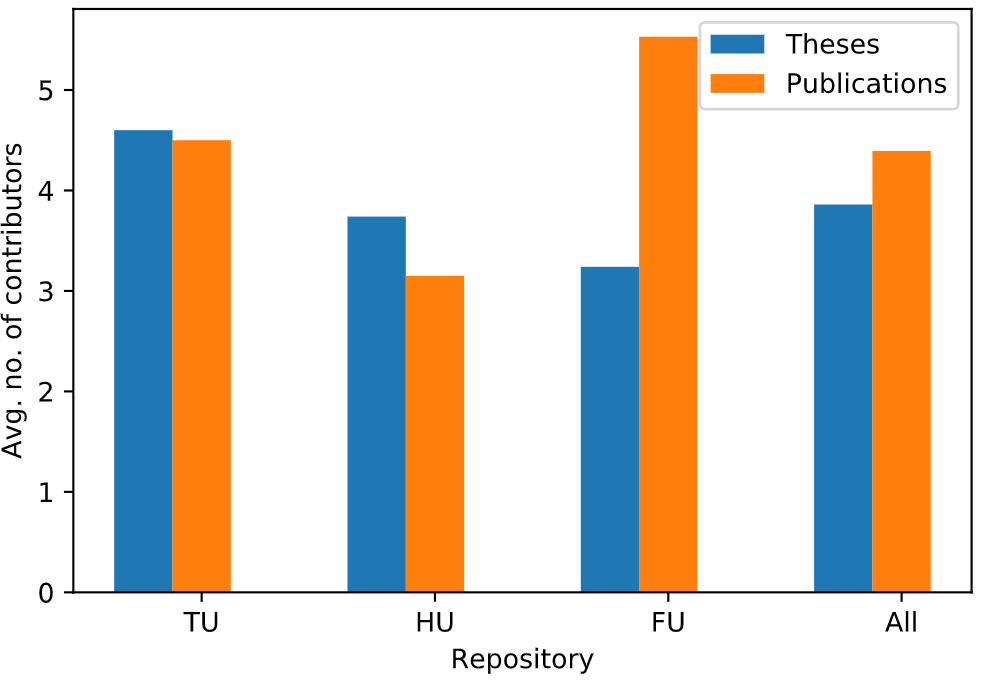
\includegraphics[width=.7\textwidth]{figures/repository_analysis/avg_contributors.PNG}
    \caption{Avg. number of contributors per document type and repository.}
    \label{fig:avg_contributors}
\end{figure}

In this section, we look at what types of contributors are present in the repositories and how often they occur. On average, documents of depositonce, edoc and refubium have 4.5, 3.4 and 4.7 contributors, respectively. In depositonce, publications and theses offer similar average numbers of contributors. In edoc, there are 0.5 more contributors in theses than in publications. In refubium it is the other way around: publications have 2.3 more contributors than theses on average. These numbers are shown illustrated in figure \ref{fig:avg_contributors}.

Regarding the types of contributors, publications usually include only the author. Edoc includes a significant number of editors, as shown in figure \ref{fig:author_types}. Theses, on the other hand, have other important types of authors: referees and advisors. After analyzing the authors, we will look at these two author types in the following sections. They are relevant because they could be used to relate documents, the same role that venues play for publications.

\begin{figure}
    \centering
    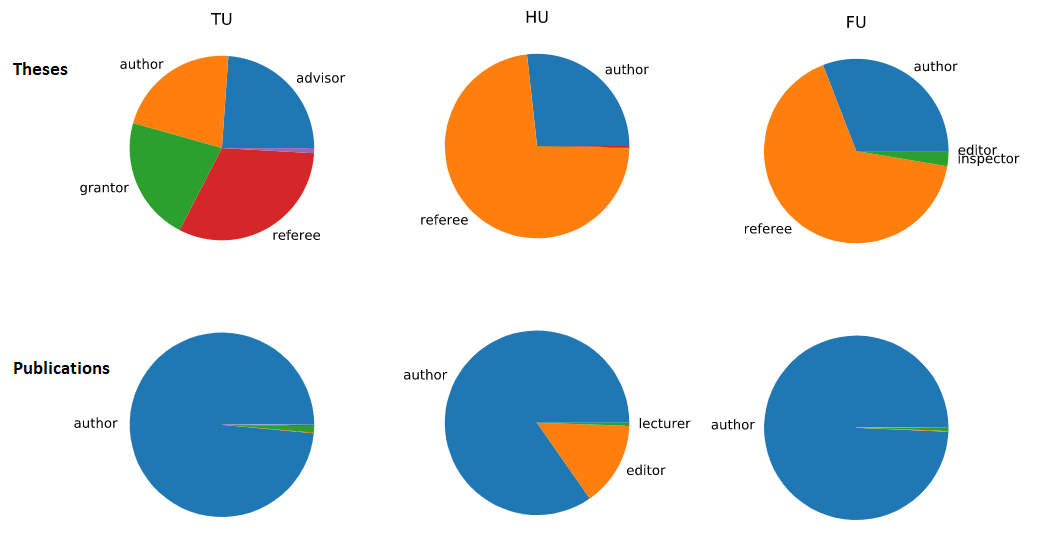
\includegraphics[width=\textwidth]{figures/repository_analysis/author_types_pretty.png}
    \caption{Author types that appear on each repository depending on the document type.}
    \label{fig:author_types}
\end{figure}


\subsubsection{Authors}

Authors are the most important contributors, as they are responsible for the content of the document. Only 207 out of the 29,399 documents don't have an author (0.7 \%), all of them being publications and 144 of them belonging to refubium. Publications have on average more authors than theses. Out of all 10,773 theses, only two of them have more than 1 author. Both of them belong to edoc. In contrast, 80 \% of the publications have multiple authors. This difference is expected, as students are usually required to write a thesis by themselves, whereas researchers often collaborate and publish their work together.

Authors of theses rarely have more than one thesis, as shown in figure \ref{fig:n_publications_per_author}. In total, 56 alumni have authored multiple theses. The real number is lower, as a quick check of some of them reveals the existence of duplicates. The ones that do have two theses to their name are Master's students that went on to pursue a PhD. On the other hand, the researchers present in the repositories have authored on average 1.6 publications. The two researchers with the most publications are Kai Nagel, from the \acrshort{tu} Berlin, and Wolfgang Härdle, from the \acrshort{hu} Berlin. Both have authored 143 publications. Still, more than 77 \% of the researchers have authored only one publication. Figure \ref{fig:n_publications_per_author} shows the distribution of researchers among the number of publications they have authored.

\begin{figure}
    \centering
    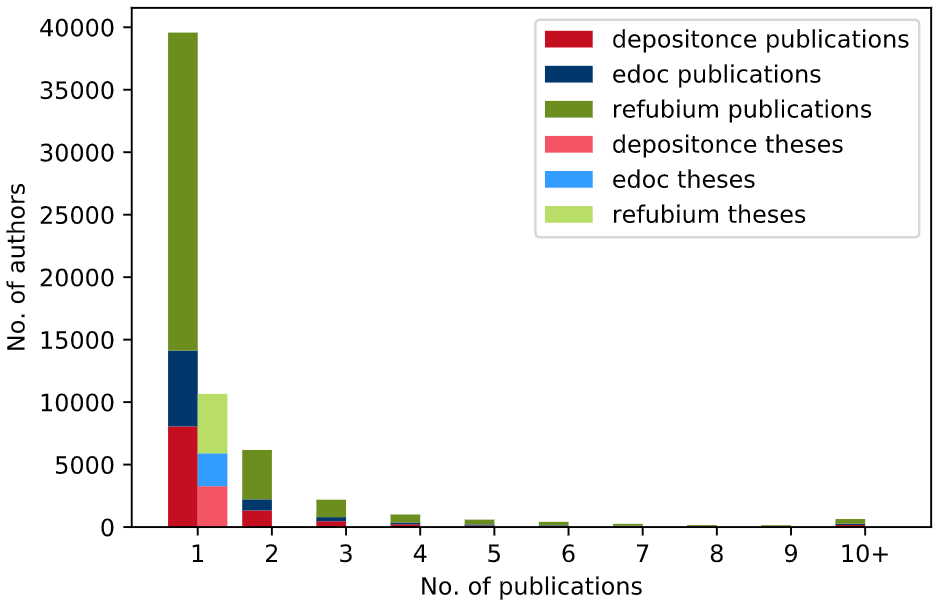
\includegraphics[width=.7\textwidth]{figures/repository_analysis/n_publications_per_author.PNG}
    \caption{No. of authors per no. of publications.}
    \label{fig:n_publications_per_author}
\end{figure}


\subsubsection{Referees}

Referees are in charge of evaluating the student's work and assigning a grade to the submitted thesis. Thus, every thesis requires at least one referee. Both edoc and refubium provide referees for almost all their theses. Only 39 and 41 documents are missing a referee, respectively. On the other hand, 1,442 theses of depositonce do not include a referee, which amounts to 19 \% of all theses.  These and all other facts presented in this section are summarized in table \ref{tab:referees}.

A caveat to the referees of refubium is the presence of ``N.N.'' as the most popular referee, appearing 1,126 times. It stands for the Latin phrase \textit{Nomen Nescio}, which means ``unknown person''. Therefore, all theses of refubium that include ``N.N.'' or variations of it can also be seen as theses without a referee. Then, refubium has 662 theses without a referee instead of 41, which amounts to 5 \% of all its theses. In total, depositonce comprises 4,780 referees, 2,388 of which are distinct. In edoc there are 7,289 referees, of which 3,390 are distinct. In refubium there are 9,133 referees and 4,863 distinct ones.

The documents that do have a referee often include more than two. On average, theses in depositonce include 2.6 referees, those of edoc 2.8 and those of refubium 2.2. Please note that theses averages don't take into account theses that have zero referees. The \textit{Nomen Nescio} referees of refubium are also ignored. The referees are professors of the universities and therefore appear frequently on the repositories, as they evaluate numerous theses. On average, professors appear two times in the repositories as referees. In depositonce there are 57 referees who have evaluated more than ten theses; in edoc there are 97 such referees and in refubium, 88. The most recurrent referees of each repository are Rupert Mutzel (FU Berlin), who has been a referee for 72 theses Wolfgang Härdle (HU Berlin), who appears on 60 theses and Peter Neubauer (TU Berlin), who appears on 45 theses.

\begin{table}[]
    \centering
    \begin{tabular}{|c|c|c|c|c|}
    \hline
         \thead{Repository} & \thead{\# referees} & \thead{\# distinct  \\ referees} & \thead{Avg. \# \\ referees \\ per thesis} & \thead{\# theses \\ without \\ a referee} \\
         \hline
         depositonce & 4,780 & 2,338 & 2.6 & 1442 (19 \%) \\
         \hline
         edoc & 7,289 & 3,390 & 2.8 & 39 (1 \%) \\
         \hline
         refubium & 9,133 & 4,863 & 2.2 & 662 (5 \%) \\
         \hline
    \end{tabular}
    \caption{Facts regarding the referees of theses.}
    \label{tab:referees}
\end{table}

\subsubsection{Advisors}

Advisors are also a building block of a thesis. They are experts on the topics handled by the thesis they advise on, and also help the student with the writing process. All facts presented in this section are summarized in table \ref{tab:advisors}. Only depositonce has a maintained list of advisors. All but 124 theses (4 \% of all theses) have at least one advisor. edoc only has 13 advisors and refubium has none. Coincidentally, depositonce is the repository where the referees are not as well maintained as in the other repositories. It seems that users of depositonce care more about advisors, and users of edoc and refubium about referees.

Students usually have just one advisor. In depositonce, theses include on average 1.1 advisors; in edoc, 1.3 advisors. Regarding how many theses share the same advisor, the average for depositonce is 3.3 theses per advisor. For edoc, the average is 1.5. Depositonce has 84 advisors that appear on more than ten different theses. edoc, on the other hand, has none. The advisor of depositonce with the most theses is Klaus-Robert Müller, who has advised 47 theses. For edoc, the most recurrent advisor is Wolfgang Härdle, who has advised 6 theses.

\begin{table}
    \centering
    \begin{tabular}{|c|c|c|c|c|}
    \hline
         \thead{Repository} & \thead{\# advisors} & \thead{\# distinct  \\ advisors} & \thead{Avg. \# \\ advisors \\ per thesis} & \thead{\# theses \\ without \\ an advisor} \\
         \hline
         depositonce & 3,603 & 1,080 & 1.1 & 124 (4 \%) \\
         \hline
         edoc & 19 & 13 & 1.3 & 2,659 (99 \%) \\
         \hline
         refubium & 0 & 0 & 0 & 4,815 (100 \%) \\
         \hline
    \end{tabular}
    \caption{Facts regarding the advisors of theses.}
    \label{tab:advisors}
\end{table}
